\documentclass[pdftex,10pt,a4paper]{article}
\usepackage[utf8]{inputenc}
\usepackage[german]{babel}
\usepackage{amsmath}
\usepackage{wrapfig}
\usepackage{listings}
\usepackage{amsfonts}
\usepackage{fontenc}
\usepackage{amssymb}
\usepackage{graphicx}
\graphicspath{ {/home/alex/github/besy/doc/images/} }
\begin{document}

\title{BS Praktikum - 2}
\author{Alex Mantel, Daniel Hofmeister}
\date{\today}
\maketitle
\newpage

\tableofcontents
\newpage

\section{Kommunikationsdiagramm}

\begin{figure}[h]
  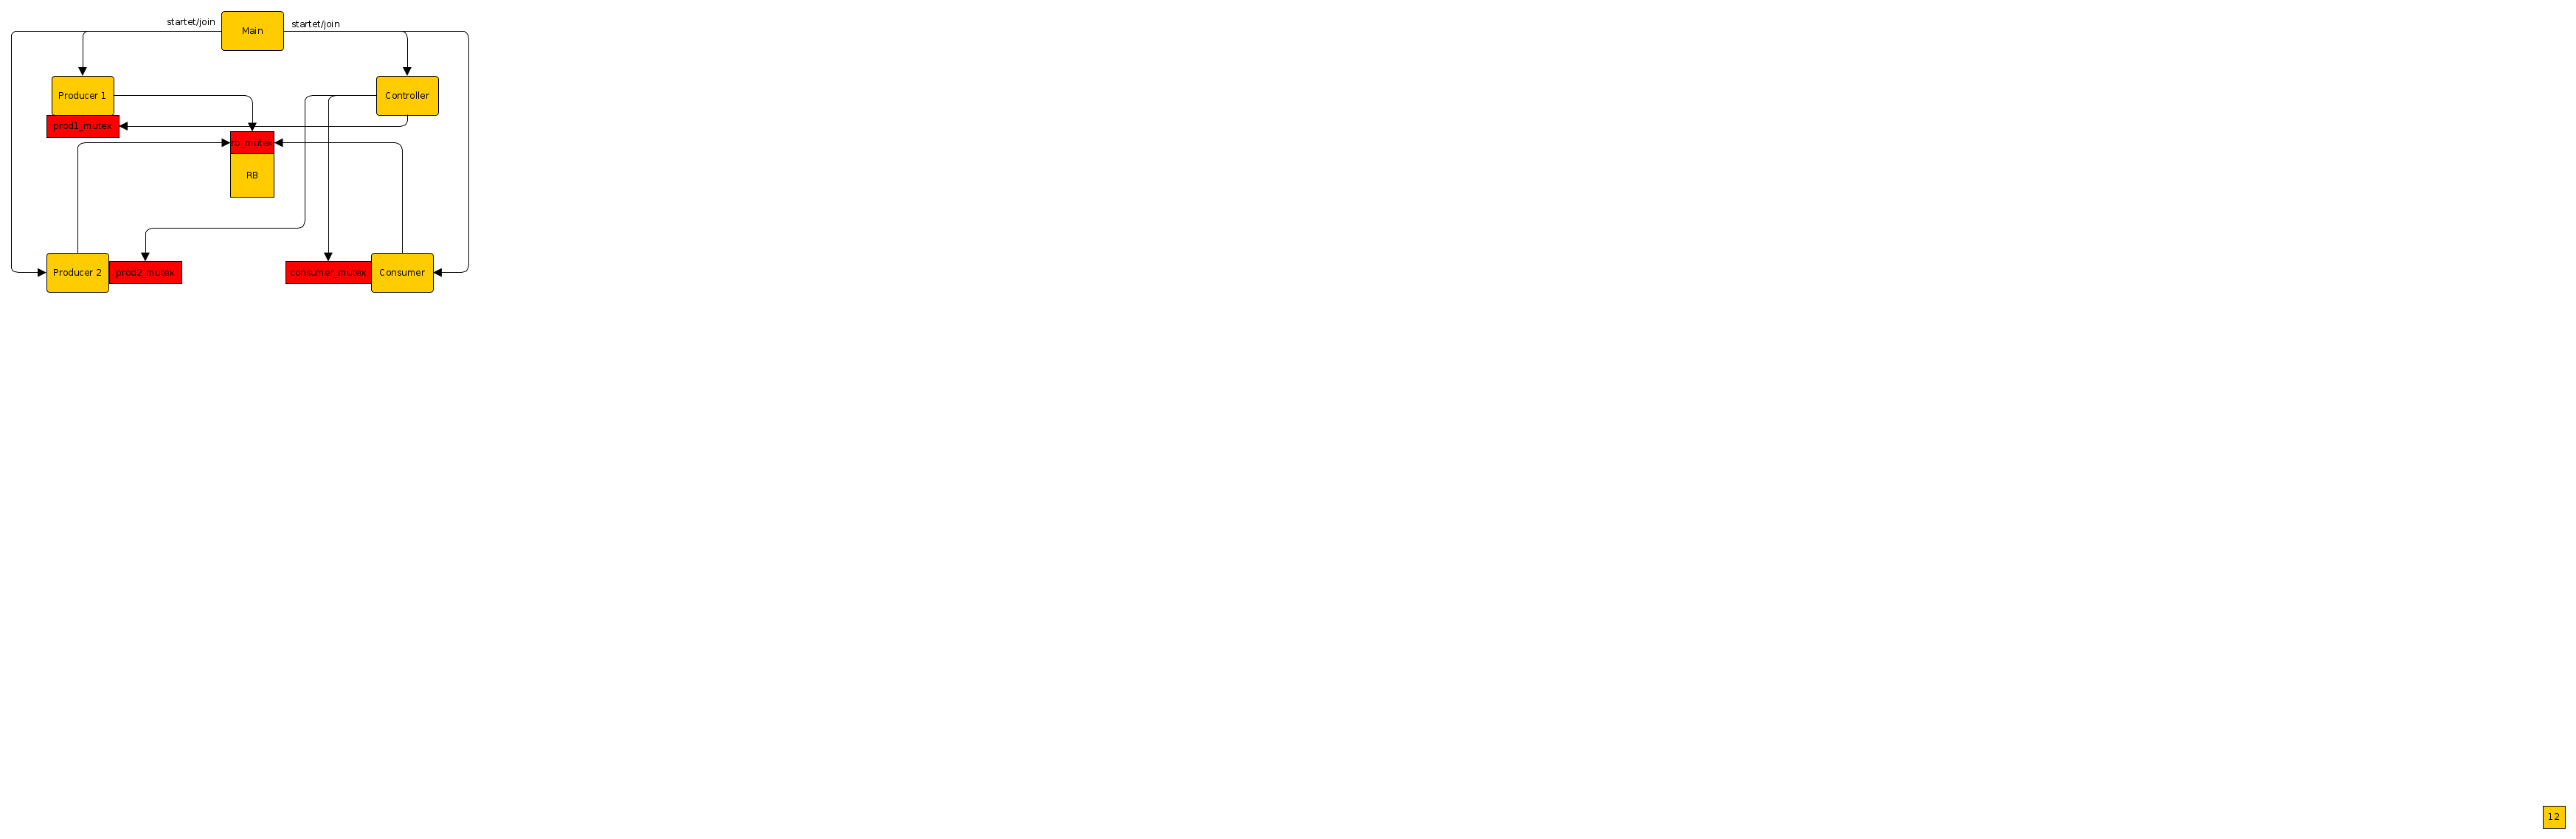
\includegraphics[scale=0.5]{kommunikation}
\end{figure}

\section{Zugeh\"origkeitstabelle}
\subsection{Mutexe}
\begin{table}[ht]
  \begin{tabular}{c | c | c | c | c}
          & rb\_mutex & prod1\_mutex & prod2\_mutex & consumer\_mutex \\
    \hline
    producer 1 &  x   &  x           &              &                 \\
    producer 2 &  x   &              &     x        &                 \\
    consumer   &  x   &              &              &    x            \\
    controller &      &  x           &     x        &    x            \\
  \end{tabular}
  \caption{Die Threads mit ihren jeweiligen Mutexen}
\end{table}

\subsection{Condition Variables}
\begin{table}[ht]
  \begin{tabular}{c | c | c | c | c | c}
          & is\_not\_full & is\_not\_empty & cond\_prod1 & cond\_prod2 & cond\_consumer \\
    \hline
    rb\_mutex      &  x  &  x  &     &     &     \\    
    prod1\_mutex   &     &     &  x  &     &     \\
    prod2\_mutex   &     &     &     &  x  &     \\
    cond\_consumer &     &     &     &     &  x  \\
  \end{tabular}
  \caption{Die Mutexe mit ihren jeweiligen Conditionvariablen}
\end{table}



\section{Pointersemantik}
Der folgende Codeausschnitt stammt aus dem Consumer und wir befinden uns in einem gelocktem Zustand. Zeile 23 verringert den counter um eins, da wir w\"ahrend der Mutex gelockt ist, einen Character auslesen. Selbes gilt f\"ur p\_out. Welcher nun erh\"oht wird um in unserem Ringbuffer auf den n\"achsten Wert zu zeigen. In den Zeilen 25 bis 27 wird \"uberpr\"uft ob der Buffer eine Runde durch ist. Hierbei sind p\_end und p\_start Macros welche auf den Anfang und das Ende des Buffers zeigen. Falls wir \"ueber die Maximalgr\"o{\ss}e des Buffers gehen, wird p\_out auf den Anfang des Buffers gesetzt damit wir unseren Ringbuffer valide halten.

\begin{lstlisting}[frame=single] 
  23     (p_rb->count)--;
  24     (p_rb->p_out)++;
  25     if((p_rb->p_out) > p_end) {
  26       p_rb->p_out = p_start;
  27     }
\end{lstlisting}

\section{Beobachtungen der Bildschirmausgabe}
W\"ahrend der Ausf\"uhrung erkennt man, dass die beiden Producer und der Consumer abwechselnd laufen. Dies mag daran liegen, dass nur jeweils einer von ihnen auf den Ringbuffer zugreifen kann. Au{\ss}erdem dachten wir, dass die Ausgabe gemischt ablaufen w\"urde. Damit meinen wir, dass der Output keinen eigenen Mutex hat und wenn zwei oder mehrere Threads eine etwas in der Kommandozeile ausgaben, sich diese Ausgaben \"uberschneiden. Nat\"urlich ist dies nicht zwischen Producer und Consumer zu erwarten. Aufgefallen ist uns dies bei Controller und Producer.

\end{document}
